%
% laserAufweiten.tex -- Bild zum Thema Optische Fouriertransformation <opt>
%
% (c) 2023 Marco Niederberger, Yanick Schoch; OST Ostschweizer Fachhochschule
%

\documentclass[tikz]{standalone}
\usepackage{times}
\usepackage{txfonts}
\usepackage{pgfplots}

\pgfplotsset{compat=1.16}
\def\skala{1}

\usetikzlibrary{arrows,intersections,math}
\usetikzlibrary{decorations.markings, calc}

%
% opt_common.tex -- Commands and color definition for the paper <opt>
%
% (c) 2023 Marco Niederberger, Yanick Schoch; OST Ostschweizer Fachhochschule
%

%%% NEW COMMANDS %%%

% Lense (x, height, curvature)
\newcommand{\lense}[3]{
    \def\curvature{0.2}
    \path[fill=glass, draw=black, line width = 0.6, opacity=0.8] (#1,-#2) .. controls (#1 - #3,0) .. (#1,#2) .. controls (#1 + #3,0) .. (#1,-#2);
}

% Dimension arrow (xStart, xEnd, yHeight, text)
\newcommand{\optMeasurement}[4]{%
    \draw[<->] (#1, #3)--(#2, #3) node[above,midway] {#4};
}

% Annotated point
\newcommand{\point}[3]{
    \draw[fill=black] (#1) circle (1pt) node[#3] {#2};
}

%%% COLORS %%%

% Define Color
\definecolor{glass}{cmyk}{0.2,0,0,0}
\colorlet{optBlue}{blue!70!black}
\colorlet{optRed}{red!90!black}

%%% STYLES %%%

% Laser rays
\tikzset{red ray/.style = {optRed, line width = 0.6}}
\tikzset{ray arrow/.style = {red ray, postaction=decorate,decoration={markings,mark=at position 0.52 with \arrow{stealth}}}}


%% Axis (x, textAbove, textBelow)
\newcommand{\xAxis}[3]{%
    \def\lenseX{2.5}
    \draw[-, thin] (#1,-\lenseX)--(#1,\lenseX) node[above]{#2};
    \node[] at (#1, -\lenseX - 0.5){#3};
}

% Styles
%% Arrow in the Middle
\tikzset{arrow inside/.style = {postaction=decorate,decoration={markings,mark=at position 0.52 with \arrow{stealth}}}}

\begin{document}

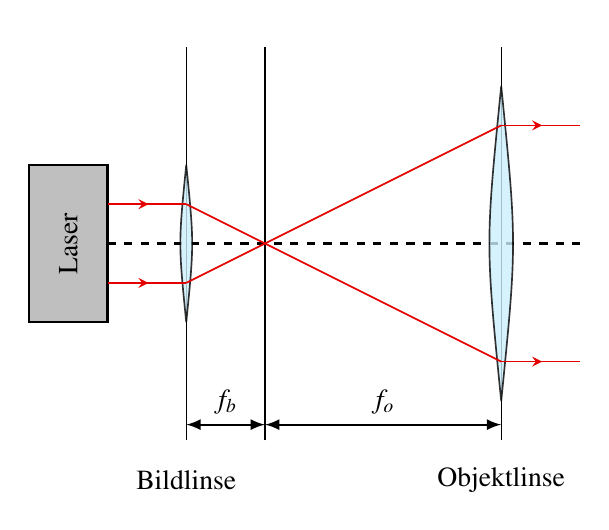
\begin{tikzpicture}[>=latex,thick,scale=\skala]

    % xAxis
    \xAxis{-1}{}{Bildlinse}
    \xAxis{0}{}{}
    \xAxis{3}{}{Objektlinse}

    % Optical plane
    \draw[dashed] (-2,0)--(4,0);

    \optMeasurement{-1}{0}{-2.3}{$f_b$}
    \optMeasurement{0}{3}{-2.3}{$f_o$}

    % Laser
    \draw[fill=lightgray] (-3, -1) rectangle (-2, 1) node[rotate=90, pos=0.5] {Laser};

    % Lenses
    \lense{-1}{1}{.1}
    \lense{3}{2}{.2}

    % Rays
    \draw[ray arrow] (-2, 0.5) -- (-1, 0.5);
    \draw[ray arrow] (-2, -0.5) -- (-1, -0.5);

    \draw[ray arrow] (3, 1.5) -- (4, 1.5);
    \draw[ray arrow] (3, -1.5) -- (4, -1.5);

    \draw[red ray] (-1, 0.5) -- (3, -1.5);
    \draw[red ray] (-1, -0.5) -- (3, 1.5);

\end{tikzpicture}
\end{document}

